\documentclass[a4paper]{ctexart}
\usepackage{xeCJK}
\usepackage{setspace}
\usepackage{graphicx,wrapfig}
\usepackage{fontspec,xunicode,xltxtra}
\usepackage{fancyhdr,titlesec,titletoc}
\usepackage[titletoc]{appendix}
\usepackage[top=29mm,bottom=29mm,left=31.8mm,right=31.8mm]{geometry}
\usepackage{enumerate,enumitem}
\usepackage{caption}
\usepackage{amsmath,amssymb,bm,array}
\usepackage{cite}
\usepackage{diagbox}
\usepackage{algorithm,algorithmicx,algpseudocode}
\usepackage{multirow}
\usepackage[super]{gbt7714}
\setmainfont{Times New Roman}
\setCJKmainfont[BoldFont={Songti SC Bold}]{SimSun}
\setCJKfamilyfont{heiti}{SimHei}
\renewcommand{\heiti}{\CJKfamily{heiti}\fontspec{Times New Roman}}
\renewcommand{\appendixpagename}{附录}

\usepackage{listings}
\usepackage[usenames,dvipsnames]{color}
\definecolor{MyDarkGreen}{rgb}{0.0,0.4,0.0}
\lstloadlanguages{Matlab}
\lstset{language=Matlab,
        frame=single,
        basicstyle=\small\ttfamily,
        keywordstyle=[1]\color{Blue}\bfseries,
        keywordstyle=[2]\color{Purple},
        keywordstyle=[3]\color{Blue}\underbar,
        identifierstyle=,
        commentstyle=\usefont{T1}{pcr}{m}{sl}\color{MyDarkGreen}\small,
        stringstyle=\color{Purple},
        showstringspaces=false,
        tabsize=5,
        morekeywords={xlim,ylim,var,alpha,factorial,poissrnd,normpdf,normcdf},
        morekeywords=[2]{on, off, interp},
        morekeywords=[3]{FindESS, homework_example},
        morecomment=[l][\color{Blue}]{...},
        numbers=left,
        firstnumber=1,
        numberstyle=\tiny\color{Blue},
        stepnumber=5
        }
\newcommand{\matlabscript}[2]
  {\begin{itemize}\item[]\lstinputlisting[caption=#2,label=#1]{#1.m}\end{itemize}}

\newcommand{\mycaptionfont}{\heiti\zihao{5}}
\captionsetup[figure]{name={\mycaptionfont 图},labelsep=period}
\captionsetup[table]{name={\mycaptionfont 表},labelsep=period}
\floatname{algorithm}{\mycaptionfont 算法}
\captionsetup[algorithm]{labelsep=period}
\renewcommand{\captionfont}{\mycaptionfont}
\renewcommand{\captionlabelfont}{\mycaptionfont}

\ctexset {
	section = {
		number = \arabic{section},
		format = \zihao{4}\bfseries,
	},
	subsection = {
		number = \arabic{section}.\arabic{subsection},
		format = \zihao{-4}\bfseries,
	},
	subsubsection = {
		number = \arabic{section}.\arabic{subsection}.\arabic{subsubsection},
		format = \zihao{-4}\bfseries,
	}
}
\setlist[enumerate]{itemindent=2em,listparindent=2em,leftmargin=0em,label=\arabic*、}

\setlength\parskip{.5\baselineskip}
\fancypagestyle{plain}{\pagestyle{fancy}}%改变章节首页页眉
\pagestyle{fancy}
\lhead{}
\chead{视觉物联网技术实验报告}
\rhead{}
\cfoot{\thepage}

\begin{document}
\begin{titlepage}
	\begin{center}
		
\includegraphics[width=0.9\textwidth]{figure//Njust.png}\\
		\vspace{10mm}
		\textbf{\zihao{2}\kaishu{物联网工程学院}}\\[0.8cm]
		\textbf{\zihao{2}\kaishu{视觉物联网技术实验报告}}\\[3cm]
		\textbf{\zihao{2}\kaishu{实验四~人脸识别 }}\\[3cm]
		\vspace{\fill}
		\setlength{\extrarowheight}{3mm}
		{\songti\zihao{3}
			\begin{tabular}{rl}
				{\makebox[4\ccwd][s]{班\qquad 级:}} & ~\kaishu 物联1601   \\
				{\makebox[4\ccwd][s]{姓\qquad 名:}} & ~\kaishu 尹达恒     \\
				{\makebox[4\ccwd][s]{学\qquad 号:}} & ~\kaishu 1030616134 \\
				{\makebox[4\ccwd][s]{指导老师:}}    & ~\kaishu 陈莹       \\
			\end{tabular}
		}\\[2cm]
		\vspace{\fill}
		\zihao{4}
		2018\textasciitilde 2019第二学期\\
		2019年5月
	\end{center}
\end{titlepage}

\renewcommand{\baselinestretch}{1.3}
\zihao{-4}
\section{实验目的}
\begin{enumerate}[label=\arabic*、]
	\item 学会使用 PCA 主成分分析法;
	\item 初步了解人脸识别的特征法;
	\item 更熟练地掌握 matlab 的使用。
\end{enumerate}

\section{实验原理}
PCA方法的基本原理是:利用离散K-L变换提取人脸的主要成分,构成特征脸空间,识别时把测试样本投影到该空间,构成一组投影系数,通过与特征脸的距离比较,距离最小的特征脸对应的即是识别结果。

基于PCA的人脸识别分为三个阶段,第一个阶段利用训练样本集构建特征脸空间;第二个阶段是训练阶段,主要是将训练图像投影到特征脸子空间上;第三个阶段是识别阶段,将测试样本集投影到特征脸子空间,然后与投影后的训练图像相比较,距离最小的为识别结果。基于PCA的人脸识别其实一种统计性的模板比配方法,原理简单,易于实现,但也有不足,它的识别率会随着关照,人脸角度,训练样本集的数量而变换,但仍不失为一种比较好的方法。


\section{实验步骤}
\subsection{图像分组}\label{sec:图像分组}
将图库中的400照片(40个个体,每个个体10张照片)分成两组。一组作为训练,一组作为测试。其中每个人的任意5张照片作为训练并作为测试样本库,其它5张作为测试待识别图片,程序如附录\ref{prog:图片整理程序}(即测试时所识别的个体出现在训练库中,后面的步骤描述和参考代码以此为基础)。

\subsection{模型训练}\label{sec:模型训练}
使用\ref{sec:图像分组}节划分得到的训练集对模型进行训练,步骤如下:
\begin{enumerate}[label=\arabic*、]
	\item 读入训练集图像并将图像全部化为一维向量,组成训练集图像矩阵;
	\item 将训练集图像矩阵中心化并计算协方差矩阵;
	\item 选取构成95\%成分的特征值;
	\item 求出原协方差矩阵的特征向量(特征脸)。
\end{enumerate}
训练程序如附录\ref{prog:训练程序}。训练完成后,使用附录\ref{prog:绘制特征脸}程序绘制前9个特征脸,结果如图\ref{figure:特征脸}。
\begin{figure}[htbp]
	\centering
	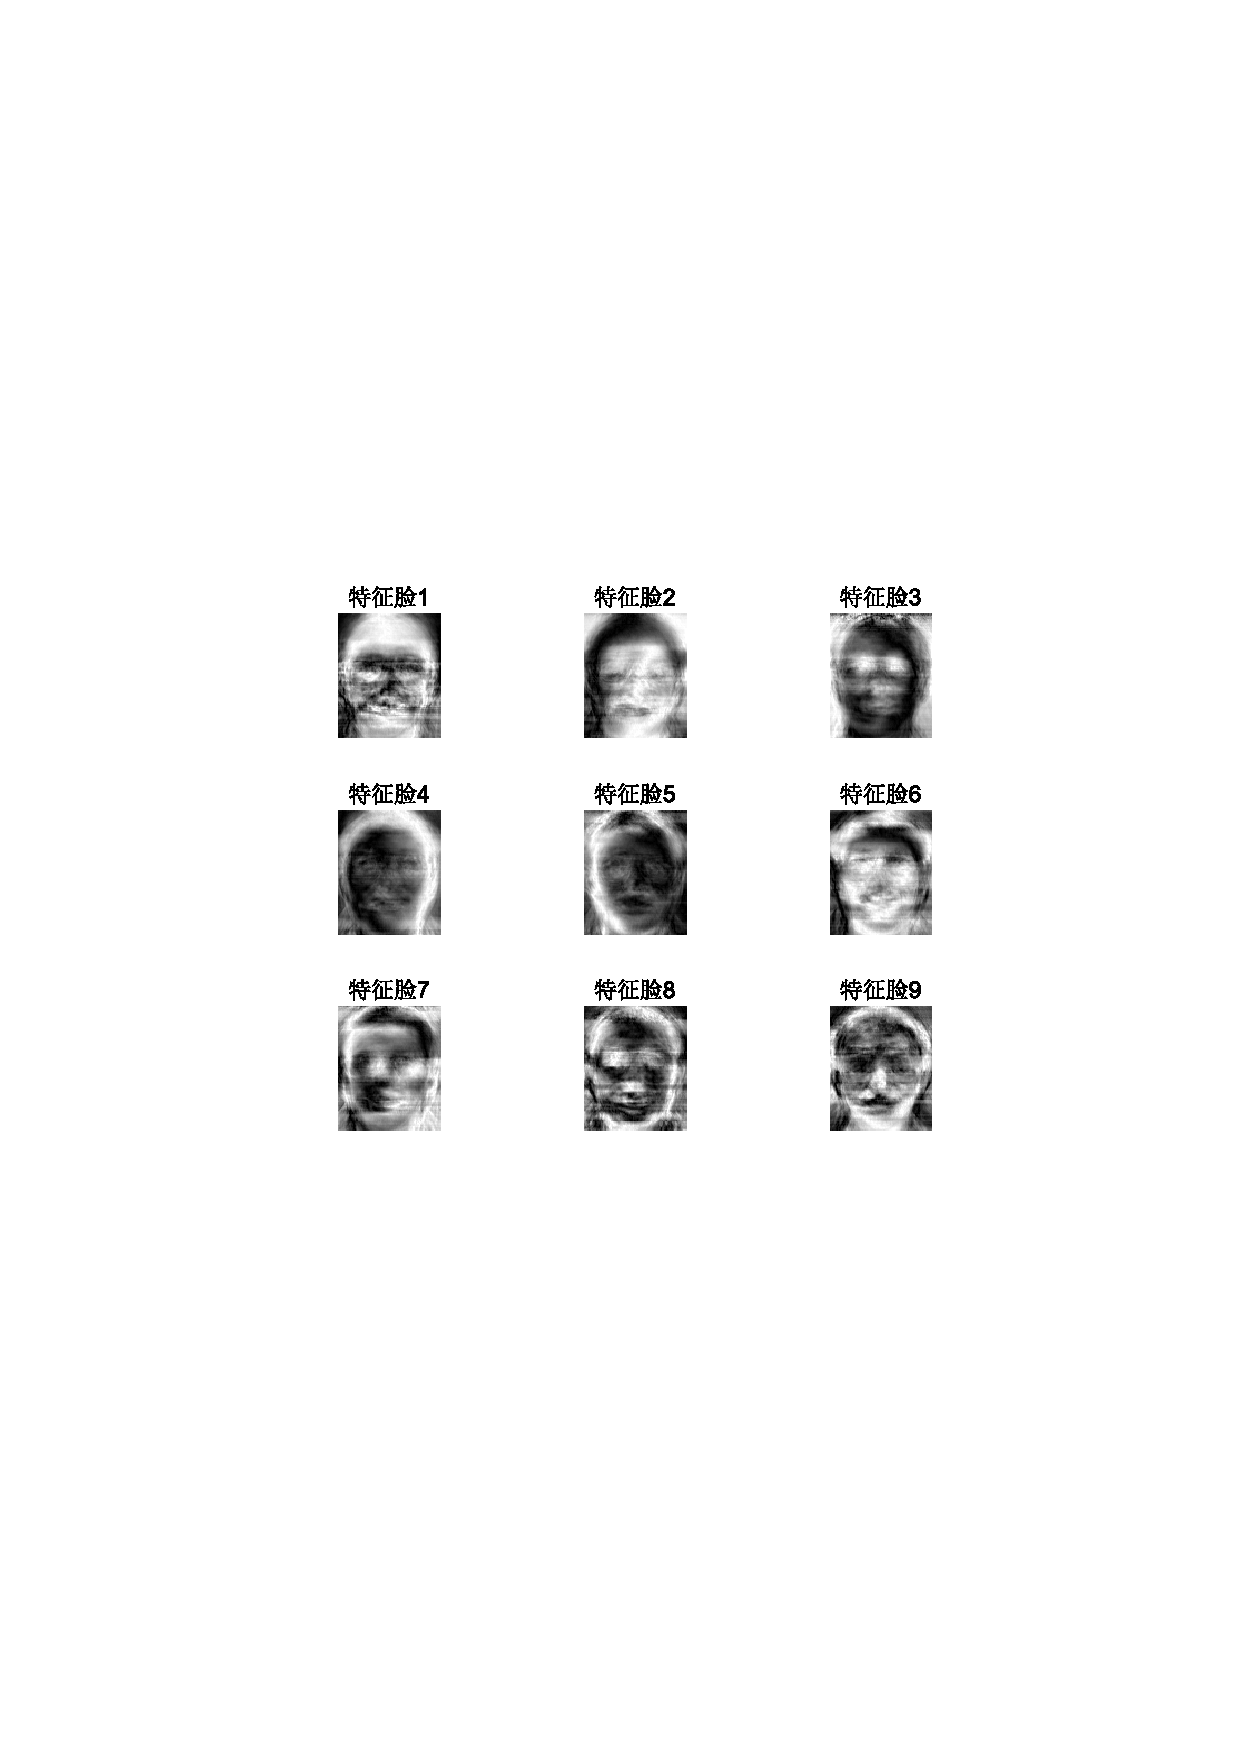
\includegraphics[width=0.8\textwidth]{figure/1.pdf}
	\caption{特征脸}\label{figure:特征脸}
\end{figure}

\subsection{模型测试}
\subsubsection{单图匹配测试}\label{sec:单图匹配测试}
使用\ref{sec:图像分组}节中所划分出的测试集的第一张图片对模型进行测试,其步骤如下:
\begin{enumerate}[label=\arabic*、]
	\item 读入测试图像;
	\item 使用\ref{sec:模型训练}节中得到的特征向量将测试图像转化为PCA特征空间下的表达矩阵;
	\item 求PCA特征空间中与测试图像最近的训练集图像;
	\item 输出该训练集图像的类别。
\end{enumerate}
按照上述思路形成附录\ref{prog:使用训练结果进行图像分类}代码;同时使用附录\ref{prog:测试程序}中的代码绘制PCA特征空间中与测试图像最近的5张训练集图像结果如图\ref{figure:单图测试}。
\begin{figure}[htbp]
	\centering
	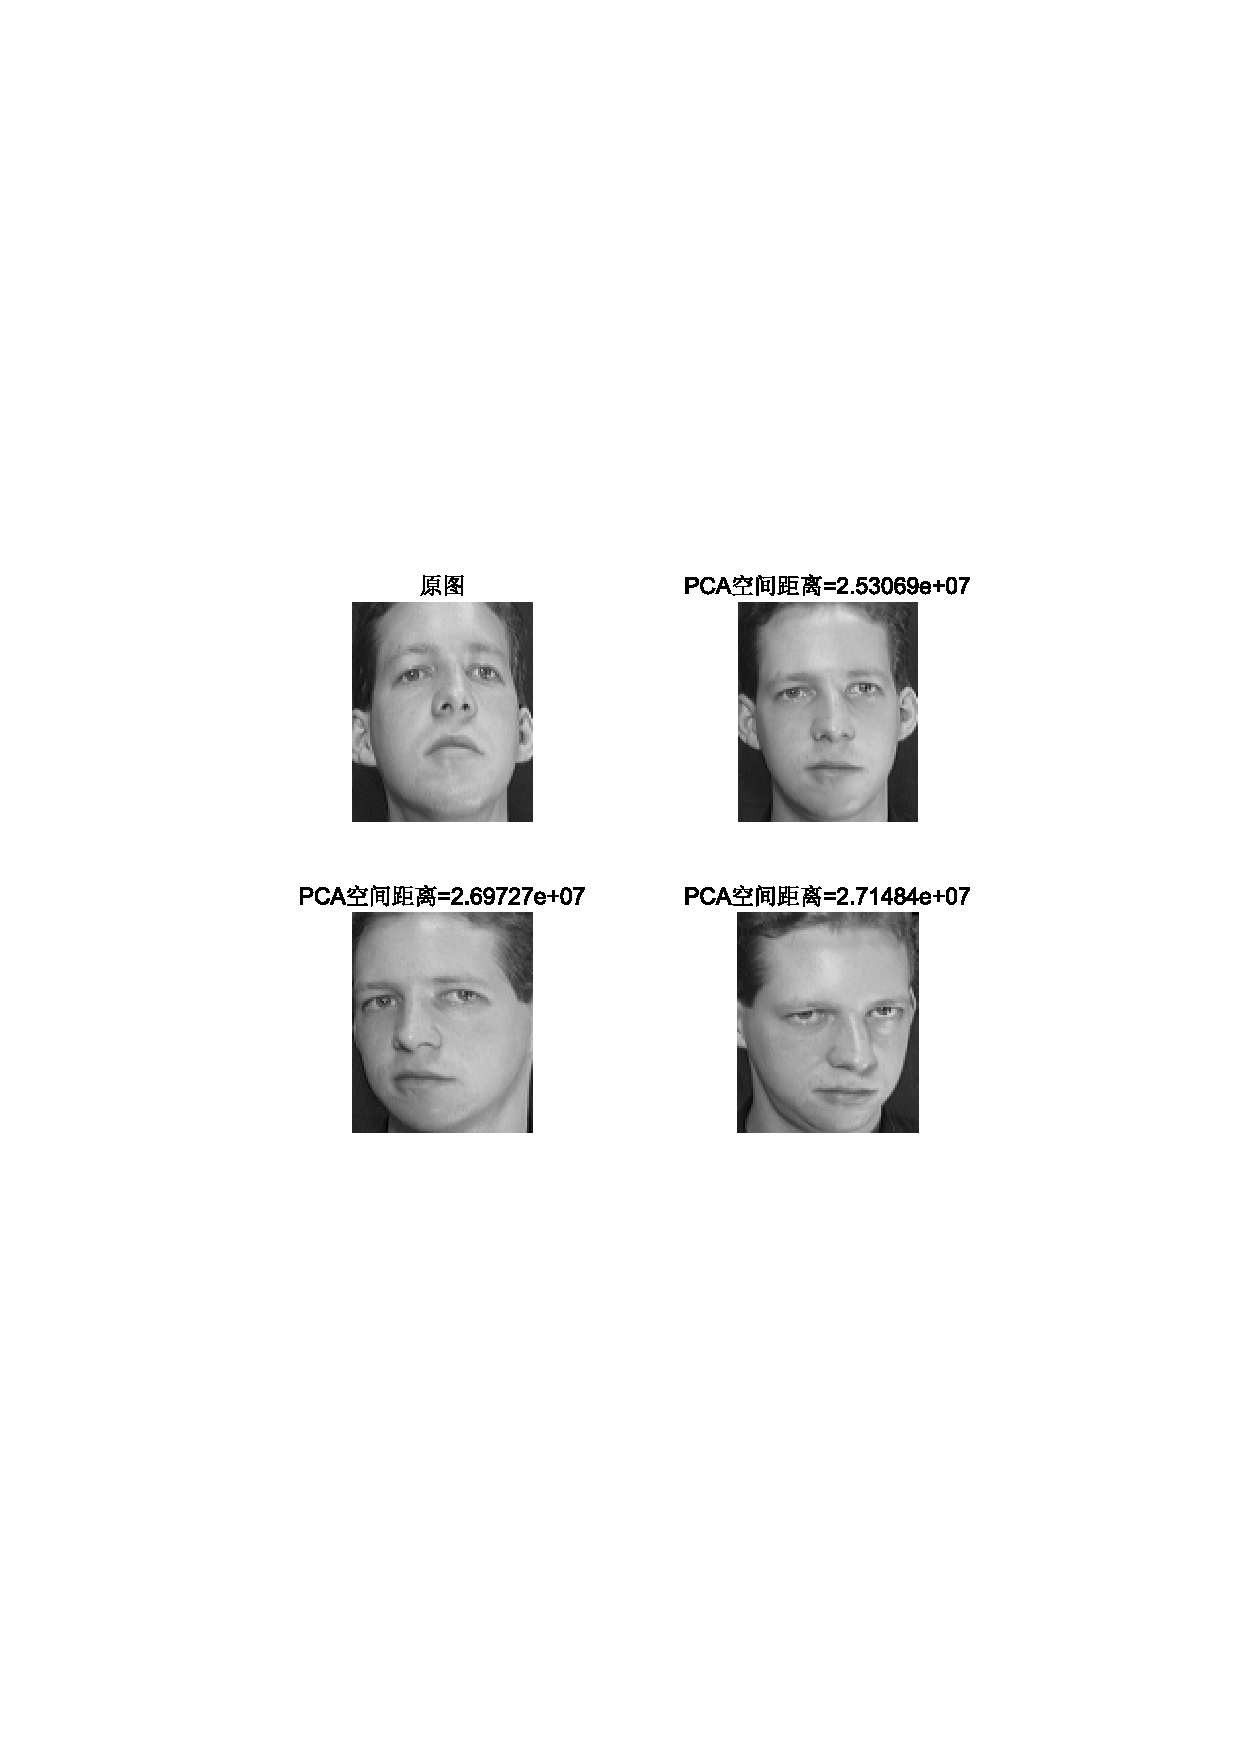
\includegraphics[width=0.8\textwidth]{figure/2.pdf}
	\caption{单图测试}\label{figure:单图测试}
\end{figure}

\subsubsection{多图准确率测试}\label{sec:多图准确率测试}
使用\ref{sec:图像分组}节中所划分出的测试集测试模型的准确率,步骤如下:
\begin{enumerate}[label=\arabic*、]
	\item 读入下一幅测试图像;
	\item 调用\ref{sec:单图匹配测试}节中的程序输出的图片类别;
	\item 比较程序输出的图片类别和图片的实际类别并记录,若训练集还要图像,则回到步骤1;
	\item 统计图片类别判定的正确率。
\end{enumerate}
其程序代码如附录\ref{prog:测试程序},运行结果为60.1\%。

\subsubsection{多数据集准确率测试}
按照\ref{sec:图像分组}中的思路使用不同的训练集和测试集图像比例进行数据集划分,并按照\ref{sec:多图准确率测试}节中的思路统计每一种划分方式下的分类准确率,对每一种训练集和测试集图像比例均进行10次实验并取均值。程序如附录\ref{prog:绘制训练集图像划分-正确率关系图},结果如图\ref{figure:训练集图像划分-正确率关系图}。
\begin{figure}[htbp]
	\centering
	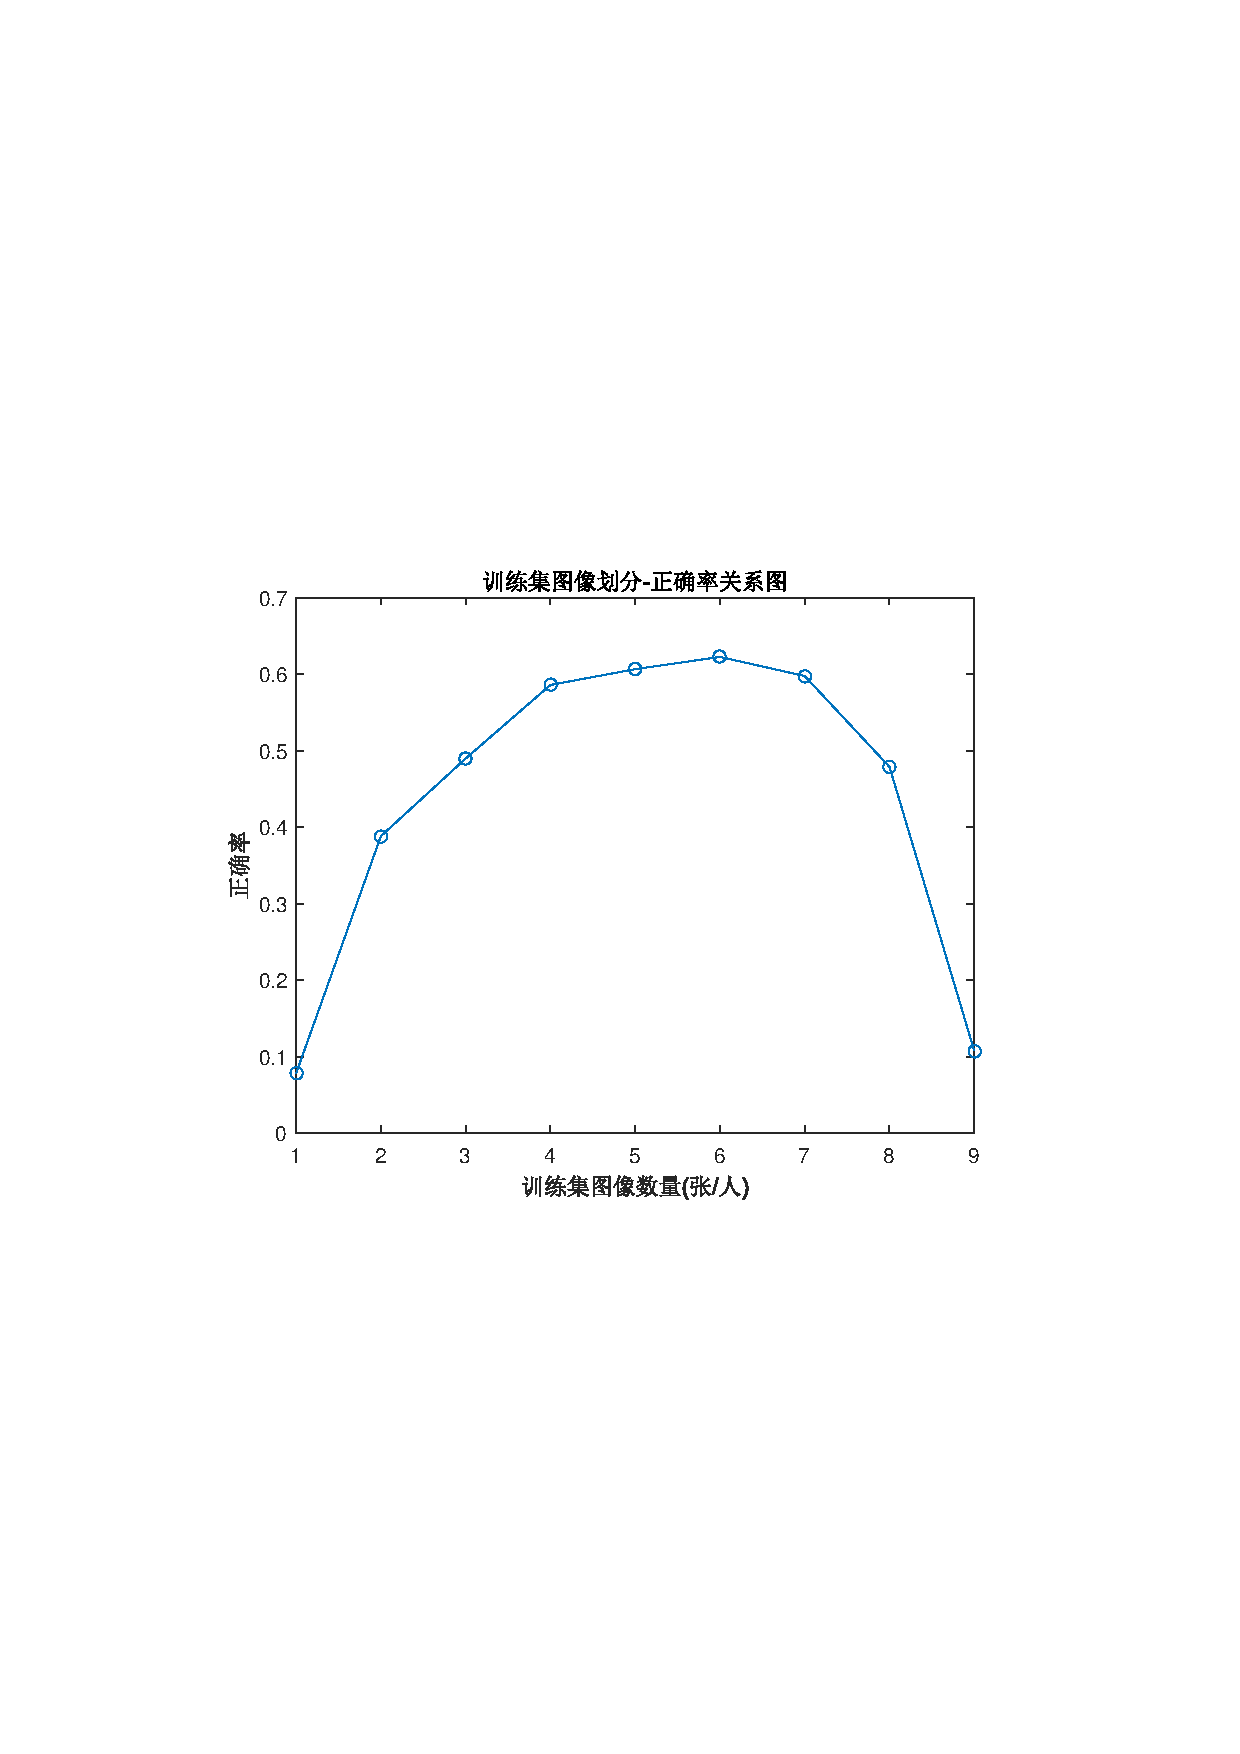
\includegraphics[width=0.8\textwidth]{figure/3.pdf}
	\caption{训练集图像划分-正确率关系图}\label{figure:训练集图像划分-正确率关系图}
\end{figure}


\section{实验结果分析}
由图\ref{figure:训练集图像划分-正确率关系图}可知,在该图像识别任务中较好的训练集-测试集图像比例在4:6$\sim$7:3之间,比例过小或过大均会对识别准确率产生不利影响。当训练集-测试集图像比例为6:4时识别准确率最高,约为62.25\%。

\newpage
\appendix
\appendixpage
\section{图片整理程序}\label{prog:图片整理程序}
\begin{lstlisting}
function setdivi(pathfrom,training_num,training_set,testing_set)
%整理图片
n = 1;
p=1;
try
rmdir(training_set, 's');
catch
end
try
rmdir(testing_set, 's');
catch
end
mkdir(training_set);
mkdir(testing_set);
for i=1:40
	a=1:10;
	Ind = a(:,randperm(size(a,2)));
	for h = 1:training_num
		j=  Ind(1,h);
		File=[pathfrom,'\s',sprintf('%d',i),'\',sprintf('%d',j),'.pgm'];
		Filesave=[training_set,sprintf('%03d',n),'.pgm'];
		copyfile(File,Filesave)
		n = n + 1;
	end
	for h = training_num+1:10
		j=  Ind(1,h);
		File=[pathfrom,'\s',sprintf('%d',i),'\',sprintf('%d',j),'.pgm'];
		Filesave=[testing_set,sprintf('%03d',p),'.pgm'];
		copyfile(File,Filesave)
		p = p + 1;
	end
end
end	
\end{lstlisting}

\section{训练程序}\label{prog:训练程序}
\begin{lstlisting}
function [ V,W,img_pj,wts ] = train( training_set )
%用训练集进行训练
path = training_set;
img_path = dir(strcat(path,'*.pgm'));
img_num = length(img_path);
imagedata = [];
if img_num >0
	for j = 1:img_num
		img_name = img_path(j).name;
		temp = imread(strcat(path, '/', img_name));
		temp = double(temp(:));
		imagedata = [imagedata, temp];
	end
end
wts = size(imagedata,2);

% 中心化并计算协方差矩阵
img_pj = mean(imagedata,2);
for i = 1:wts
	imagedata(:,i) = imagedata(:,i) - img_pj;
end
covMat = imagedata'*imagedata;

[COEFF, latent, explained] = pcacov(covMat);
% 选择构成 95%能量的特征值
i = 1; proportion = 0;
while(proportion < 95)
	proportion = proportion + explained(i);
	i = i+1;
end
k = i - 1;
%求出原协方差矩阵的特征向量,即特征脸
V = imagedata*COEFF;
% N*M 阶
V = V(:,1:k);
% 训练样本在 PCA 特征空间下的表达矩阵 k*M
W = V'*imagedata;
disp('训练完成');
end	
\end{lstlisting}

\section{绘制特征脸}\label{prog:绘制特征脸}
\begin{lstlisting}
function test( img_path,training_set,V,W,img_pj,wts )
%测试
im=imread(img_path);
subplot(2,2,1);
imshow(im);
title('原图');
im = double(im(:));
objectone = V'*(im - img_pj);
temp=[];
for k = 1:wts
	temp(k) = norm(objectone - W(:,k));
end
[s_temp,id]=sort(temp,'ascend');

for i=1:3
	subplot(2,2,i+1);
	imshow(imread([training_set,sprintf('%03d.pgm',id(i))]));
	title(sprintf('PCA空间距离=%g',s_temp(i)));
end
end
\end{lstlisting}

\section{使用训练结果进行图像分类}\label{prog:使用训练结果进行图像分类}
\begin{lstlisting}
function c = classify(im,V,W,img_pj,wts)
im = double(im(:));
objectone = V'*(im - img_pj);
c=0;
m=inf;
for k = 1:wts
    t=norm(objectone - W(:,k));
    if t<m
        m=t;
        c=k;
    end
end
end
\end{lstlisting}

\section{统计正确率}
\begin{lstlisting}
function a = accurancy( testing_set,V,W,img_pj,wts,training_num )
%计算正确率
path = testing_set;
img_path = dir(strcat(path,'*.pgm'));
img_num = length(img_path);
if img_num >0
	total=0;
	testing_num=10-training_num;
	for j = 1:img_num
		img_name = img_path(j).name;
		im = imread(strcat(path, '/', img_name));
		c=classify(im,V,W,img_pj,wts);
		if floor(c/training_num)==floor(j/testing_num)
			total=total+1;
		end
		a=total/img_num;
	end
end
end
\end{lstlisting}

\section{测试程序}\label{prog:测试程序}
\begin{lstlisting}
clear;
pathfrom='images';
training_num=5;
training_set='sets/training/';
testing_set='sets/testing/';
setdivi(pathfrom,training_num,training_set,testing_set);
[ V,W,img_pj,wts ] = train( training_set );

faces=zeros(112,92,0);
for i=1:size(V,2)
	temp=V(:,i);
	faces(:,:,end+1)=mapminmax(reshape(temp,[112,92]),0,1);
end
for i=1:9
	subplot(3,3,i)
	imshow(faces(:,:,i));
	title(sprintf('特征脸%d',i))
end

test( [testing_set,'001.pgm'],training_set,V,W,img_pj,wts );

a=accurancy(testing_set,V,W,img_pj,wts,training_num);

fprintf('正确率为%f\n',a);
\end{lstlisting}

\section{绘制训练集图像划分-正确率关系图}\label{prog:绘制训练集图像划分-正确率关系图}
\begin{lstlisting}
clear;
pathfrom='images';
x=1:9;
y=[];
for training_num=x
    training_set=sprintf('sets/training%d/',training_num);
    testing_set=sprintf('sets/testing%d/',training_num);
    k=10;
    a=0;
    for i=1:k
        setdivi(pathfrom,training_num,training_set,testing_set);
        [ V,W,img_pj,wts ] = train( training_set );
        a = a+ accurancy( testing_set,V,W,img_pj,wts,training_num );
    end
    y(end+1)=a/k;
end
plot(x,y,'marker','o')
xlabel('训练集图像数量(张/人)');
ylabel('正确率');
title('训练集图像划分-正确率关系图');
\end{lstlisting}

\end{document}